%%%%%%%%%%%%%%%%%%%%%%%%%%%%%%%%%%%%%%%%%
% Thin Sectioned Essay
% LaTeX Template
% Version 1.0 (3/8/13)
%
% This template has been downloaded from:
% http://www.LaTeXTemplates.com
%
% Original Author:
% Nicolas Diaz (nsdiaz@uc.cl) with extensive modifications by:
% Vel (vel@latextemplates.com)
%
% License:
% CC BY-NC-SA 3.0 (http://creativecommons.org/licenses/by-nc-sa/3.0/)
%
%%%%%%%%%%%%%%%%%%%%%%%%%%%%%%%%%%%%%%%%%

%----------------------------------------------------------------------------------------
%	PACKAGES AND OTHER DOCUMENT CONFIGURATIONS
%----------------------------------------------------------------------------------------

\documentclass[a4paper, 11pt]{article} % Font size (can be 10pt, 11pt or 12pt) and paper size (remove a4paper for US letter paper)

\usepackage[protrusion=true,expansion=true]{microtype} % Better typography
\usepackage{graphicx} % Required for including pictures
\graphicspath{{images/}}
\usepackage{wrapfig} % Allows in-line images

\usepackage{amsmath} 
\usepackage{mathpazo} % Use the Palatino font
\usepackage[T1]{fontenc} % Required for accented characters
\linespread{1.05} % Change line spacing here, Palatino benefits from a slight increase by default

\makeatletter
\renewcommand\@biblabel[1]{\textbf{#1.}} % Change the square brackets for each bibliography item from '[1]' to '1.'
\renewcommand{\@listI}{\itemsep=0pt} % Reduce the space between items in the itemize and enumerate environments and the bibliography

\renewcommand{\maketitle}{ % Customize the title - do not edit title and author name here, see the TITLE block below
\begin{flushright} % Right align
{\LARGE\@title} % Increase the font size of the title

\vspace{50pt} % Some vertical space between the title and author name

{\large\@author} % Author name
\\\@date % Date

\vspace{40pt} % Some vertical space between the author block and abstract
\end{flushright}
}

%----------------------------------------------------------------------------------------
%	TITLE
%----------------------------------------------------------------------------------------

\title{\textbf{High Frequency Transformer Design Report}\\ % Title
Consultancy Report} % Subtitle

\author{\textsc{Ozan Keysan} % Author
\\{\textit{University of Edinburgh}}} % Institution

\date{\today} % Date

%----------------------------------------------------------------------------------------

\begin{document}

\maketitle % Print the title section

%----------------------------------------------------------------------------------------
%	ABSTRACT AND KEYWORDS
%----------------------------------------------------------------------------------------

%\renewcommand{\abstractname}{Summary} % Uncomment to change the name of the abstract to something else

\begin{abstract}
I think we agreed the report would be submitted on 14 May and cover: Magnetic formula and limitations, electric formula and limitations and physical limitations.

The aim of this report


\end{abstract}

\hspace*{3,6mm}\textit{Keywords:} lorem , ipsum , dolor , sit amet , lectus % Keywords

\vspace{30pt} % Some vertical space between the abstract and first section

%----------------------------------------------------------------------------------------
%	ESSAY BODY
%----------------------------------------------------------------------------------------

\section*{Introduction}



\subsection{AC Winding Losses}

The high frequency excitation has two main effects in the transformer windings:
\begin{itemize}
  \item Skin Effect: In AC excitation the current itself generates an opposing magnetic field and current, which reduce the net current density inside the conductor. The total current will stay same, but the distribution will be higher across the circumference of the conductor.
  \item Proximity Effect is the interaction between two adjacent conductors that alters the current distribution in the conductor. Same principles(e.g. proximity, frequency) apply in the proximity affect.
\end{itemize}

Foil conductors are favoured in primary windings of high frequency transformers as the conductor thickness can be reduced while achieving a high cross-section area.

Dowell calculated eddy losses in transformer windings in \cite{Dowell1966}. A detailed explanation of these one dimensional Maxwell equations can be found in \cite{Villar2010}. Referring those equations, the DC resistance of a foil winding can be expressed as:

\begin{equation}
  R_{dc} = \rho \frac{L_{mean}}{t_w h_w} N_{turns}
\end{equation}

where $L_{mean}$ is the mean turn length of the coil, $t_w$ is the thickness, $h_w$ is the height, $\rho$ is the resistivity of copper.

The AC resistance is more complicated and depends on the ratio of the wire thickness to skin depth ($\delta$):

\begin{equation}
  R_{ac}=\rho \frac{L_{mean}}{h_w \delta} N_{turns} \left[\varsigma_1 + \frac{2}{3} (N_{turns}^2-1)\varsigma_2\right]
\end{equation}
where:

\begin{equation}
  \varsigma_1 = \dfrac{sinh(2\Delta)+sin(2\Delta)}{cosh(2\Delta)-cos(2\Delta)} \quad
  \varsigma_2 = \dfrac{sinh(\Delta)-sin(\Delta)}{cosh(\Delta)+cos(\Delta)} \quad  
  \Delta = \dfrac{t_w}{\delta}
\end{equation}

Thus, the important factor is the penetration factor (i.e the ratio of conductor thickness to skin depth, $\Delta$). The ratio of AC resistance to DC resistance is called Dowell's resistance factor ($F_r$). The resistance factor as a function of penetration ratio for a 2 mm thick foil wire is presented in Fig.~\ref{resistance_factor}. For example, at 1 kHz the skin depth is 2.1 mm (the penetration ratio is approximately 1), the resistance factor is 2.7 for a layer number of 4. Thus the resistive losses will be 2.7 times more compared to DC conduction.

\begin{figure}[]
  \centering
    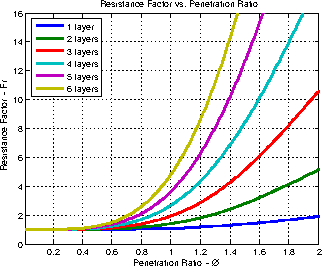
\includegraphics[scale=1.25]{resistance_factor}
  \caption{Resistance factor for a function of penetration ratio (for 2 mm thick foil conductor) \cite{Villar2010}.}
  \label{resistance_factor}
\end{figure}


!! Secondary winding factorunu karsilastir
\cite{Sullivan2003,Ferreira1994} makalelerini oku

%----------------------------------------------------------------------------------------
%	BIBLIOGRAPHY
%----------------------------------------------------------------------------------------

\bibliographystyle{unsrt}

\bibliography{../refler/NAREC}

%----------------------------------------------------------------------------------------

\end{document}